%% 7.5 %%

\section{The Fundamental Theorem of Calculus}
\setcounter{exercise}{0}

\bx{
If $f$ is continuous, then we know from Theorem 7.2.9
that is is integrable. 

Then, from the Fundamental Theorem of Calculus,
that we can define
\begin{equation*}
  F(x) = \int_a^x f,
\end{equation*}
where $F'(c) = f(c)$ at all the continuous points of $f$.
This means $f$ is the derivative of $F$.
}

\bx{
\ea{
\item For $x \in [-1, 0]$, we just have 
\begin{equation*}
  F(x) 
  = \frac{
    (-x+1)(x+1)
  }{2}
  = \frac{
    1-x^2
  }{
    2
  }
\end{equation*}
For $x \in (-\infty, 1)$, 
\begin{equation*}
  F(x) = 
  \frac{
    (-1-x)(-1-x)
  }{
    2
  }
  = \frac{
    1-x^2
  }{
    2
  }
\end{equation*}
and for 
$x \in (1, \infty)$, we have 
\begin{equation*}
  F(x) = \frac{1}{2} + \frac{x^2}{2}
\end{equation*}
Putting these together gives 
\begin{equation*}
  F(x) = \begin{cases}
    \frac{1-x^2}{2}, &x \leq 0\\
    \frac{1+x^2}{2}, &x \geq 0
  \end{cases}
\end{equation*}
See Figure 
\ref{chap7:fig:Fx_final}
for the plot of $F(X)$.

I computed these by geometrically looking at the area of a trapezoid.
See Figure
\ref{chap7:fig:calculating_integral}
for more details.

\begin{figure}[H]
  \centering
  \subfloat[Finding $F(x)$]{
    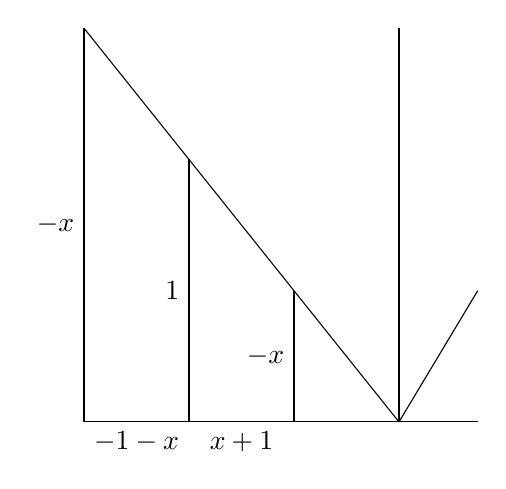
\begin{tikzpicture}
      \draw 
        (0,0) -- (0, 5)
        (0,0) -- (1, 0)
        (0,0) -- (-4, 0)
      ;

      \draw
        (0,0) -- (-4, 5)
        (0,0) -- (1, 5/3)
      ;

      \draw 
        (-4, 0) -- (-4, 5)
        (-8/3, 0) -- (-8/3, 10/3)
        (-4/3, 0) -- (-4/3, 5/3)
      ;

      \draw 
        (-4, 2.5) node[left] {$-x$}
        (-8/3, 5/3) node[left] {1}
        (-4/3, 5/6) node[left] {$-x$}
      ;

      \draw
        (-10/3, 0) node[below] {$-1-x$}
        (-2, 0) node[below] {$x+1$}
      ;
    \end{tikzpicture}
    \label{chap7:fig:calculating_integral}
  }
  \qquad
  \subfloat[$F(x)$]{
    \begin{tikzpicture}
      \begin{axis}[
          axis lines = center,
          xlabel = $x$,
          ylabel = {$F(x)$},
      ]

      \addplot[
          domain=0:3, 
          samples=100, 
          color=red
      ]{
        0.5*x^2 + 1/2
      };
      \addlegendentry{$x \geq 0$}

      \addplot[
          domain=-3:0, 
          samples=100, 
          color=blue
      ]{
        -0.5*x^2 + 1/2
      };
      \addlegendentry{$x \leq 0$}
      \end{axis}
    \end{tikzpicture}
    \label{chap7:fig:Fx_final}
  }
  \caption{}
\end{figure}

$F$ is continuous everywhere, and differentiable everywhere.
Therefore, $F'(x) = f(x)$ everywhere as well.

\item 
}
}